\chapter{Hardware}

\par En este capítulo se analiza el componente electrónico o de hardware, de aquí en mas, estación de recolección de datos. Se aborda la elección de los elementos que la componen, el diseño de interconexión, y la descripción del software que se ejecuta dentro de la misma. Detallándose, en esta última, las funcionalidades de obtención y persistencia de datos necesarias para el funcionamiento de la estación.

\section{Tecnologías evaluadas}
    \par Para el funcionamiento del prototipo propuesto es necesario obtener datos digitales provenientes de múltiples sensores\footnote{Dispositivo diseñado para recibir información de una magnitud del exterior y transformarla en otra magnitud, normalmente eléctrica, que seamos capaces de cuantificar y manipular} (temperatura y pH de líquidos;  temperatura y humedad ambiental); disponer de capacidad de almacenamiento para la persistencia de datos; e incorporar conectividad para transmisión de datos. De forma adicional, el componente debe poseer un tamaño reducido, de manera de no estorbar en las actividades de producción.

    \par Existen diferentes plataformas dentro de las cuales puede ser desarrollado un componente que cumpla los requerimientos antes mencionados. Raspberry\textsuperscript{\textregistered} y Arduino\textsuperscript{\textregistered} se destacan como las más utilizadas y con mayor comunidad, por tanto, luego se describen y comparan en detalle.
    
    \par Respecto de la recolección de datos, los sensores se describen abordando aspectos como costo económico, precisión y fiabilidad de los datos.
    
    \subsection{Análisis de elementos}
        \subsubsection{Arduino: Microcontrolador}
            \par Arduino\textsuperscript{\textregistered} es una compañía de cultura libre\footnote{Corriente de pensamiento que promueve la libertad en la distribución y modificación de trabajos creativos basándose en el principio del contenido libre para distribuir o modificar trabajos y obras creativas.} que manufactura placas de desarrollo de hardware para construir dispositivos digitales e interactivos que pueden sensar y controlar objetos del mundo real. 
 
            \par El software de Arduino\textsuperscript{\textregistered} consiste de dos elementos, un entorno de desarrollo (IDE) y un bootloader que es ejecutado de forma automática dentro del microcontrolador en cuanto este se enciende. Las placas Arduino se programan mediante un computador, usando comunicación serial.
        
            \par Generalmente el hardware (Figura \ref{boardArduino}) consiste de un microcontrolador Atmel AVR, conectado sobre una placa de circuito impreso con al menos 16 GPIO (\textit{General Purpose Input Output}) para entrada y salida de datos. A la misma se le pueden conectar placas de expansión (shields) que complementan la funcionalidad del modelo de placa empleada, agregando circuiteria, sensores y módulos de comunicación externos a la placa original.
        
            \begin{figure}[h]
                \centering
                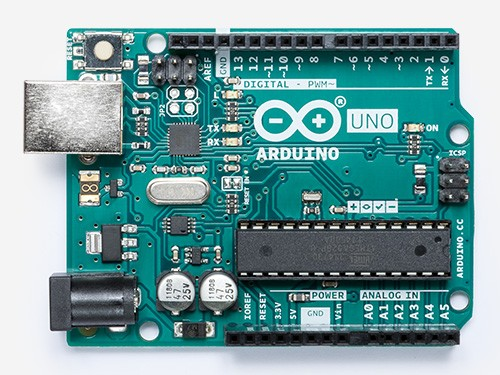
\includegraphics[scale=0.6]{hardware/Arduino.jpg}
                \caption{Placa Arduino\textsuperscript{\textregistered} UNO}
                \label{boardArduino}
            \end{figure}
        
        \subsubsection{Raspberry: Computadora de placa reducida}
            \par Raspberry\textsuperscript{\textregistered} Pi es un computador de placa reducida, computador de placa única o computador de placa simple (SBC) de bajo costo. Es desarrollado en Reino Unido por la Fundación Raspberry\textsuperscript{\textregistered} Pi.
        
            \par El software es open source, siendo su sistema operativo oficial una versión adaptada de Debian, denominada Raspbian. También, permite usar otros sistemas operativos, incluido una versión de Windows 10.
        
            \par El hardware (Firgura \ref{boardRaspberry}), en todas sus versiones, incluye un procesador Broadcom, una memoria RAM, una GPU, puertos USB, HDMI, Ethernet y 40 pines GPIO. Ninguna de sus ediciones incluye memoria de almacenamiento pero si cuentan con un slot para memoria MicroSD. Ofrece, en forma adicional, la posibilidad de agregar placas de expansión llamadas HAT (Hardware Attached on Top) para agregar otras funcionalidades.
            
            \begin{minipage}{0.95\textwidth}
            
            \begin{center}
                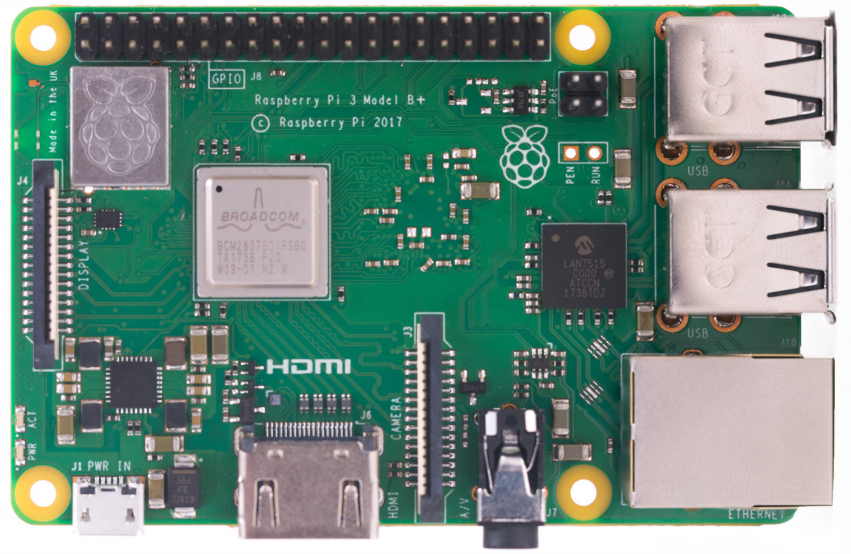
\includegraphics[scale=0.30]{hardware/raspberrypib3.jpg}
                
                \captionof{figure}{Placa Raspberry\textsuperscript{\textregistered} pi 3 B+}
                \label{boardRaspberry}
            \end{center}
            \end{minipage}
            \begin{minipage}{0.95\textwidth}
            \subsubsection{Comparación}
                \par En la Tabla \ref{CompHard}, se puede observar la comparación entre las dos placas descritas en la sección anterior. Los criterios de comparación utilizados se enfocaron en los requerimientos que este proyecto posee sobre dichos componentes.
            \end{minipage}
        
            
            \begin{center}
            \begin{tabularx}{\textwidth}{| X | X | X |}
            \hline
            \multicolumn{3}{|c|}{\textbf{Comparación Plataformas de Hardware}} \\
            \hline
            Criterio de Comparación & Arduino\textsuperscript{\textregistered} & Raspberry\textsuperscript{\textregistered} pi \\
            \hline
            \hline
        
            Precio & \$440 (USD 17,00) & \$1900 (USD 61,00)
            \\ \hline
            Manejo de sensores & Digitales y analógicos & Digitales y analógicos
            \\ \hline
            Capacidad de procesamiento, memoria y almacenamiento & Procesador de 8 bits a 16Mhz, memoria de 2KB, sin almacenamiento (sin slot de expansión). & Procesador de 64 bits a 1.4Ghz, memoria de 1GB, sin almacenamiento (Slot memoria SD).
            \\ \hline
            Conectividad & Conexión USB (tipo B) x 1. Pueden adicionarse Shields Ethernet, Bluetooth o WiFi. & Conexión USB (tipo A) x 4, Ethernet 100M, WiFi 802.11n/ac, Bluetooth.
            \\ \hline
            Tamaño & 7.6 x 1.9 x 6.4 cm. & 8.6cm x 5.4cm x 1.7cm.
            \\ \hline
            Lenguaje de programación & Lenguaje Bajo Nivel. Gran comunidad y soporte. Se requiere de un computador para el desarrollo. & Lenguaje Alto Nivel. Gran comunidad y soporte. Se desarrolla directamente en el dispositivo.
            \\ \hline
            Persistencia de datos ante pérdida de alimentación eléctrica & Ninguna & Al utilizar una memoria SD, se obtiene persistencia de datos.
            \\
            \hline
            \end{tabularx}
            \label{CompHard}
            \captionof{table}{Comparación entre Arduino y Raspberry Pi}
            \end{center}
            
        
    \subsection{Elementos utilizados}
        \par A continuación se detallan los componentes de hardware utilizados.
        
        \subsubsection{Placa electrónica}
            \par En base al análisis de la Tabla \ref{CompHard}, la tecnología utilizada en este proyecto es \textbf{Raspberry\textsuperscript{\textregistered} Pi} (modelo Raspberry\textsuperscript{\textregistered} Pi 3 B+) debido a la mayor capacidad de procesamiento, almacenamiento, persistencia de datos y el lenguaje de programación de alto nivel. Como esta placa incorpora conectividad inalámbrica de fábrica, posee la ventaja sobre Arduino\textsuperscript{\textregistered} de no requerir la instalación de placas externas para este fin, siendo este tipo de conexiones necesarias para el desarrollo de este proyecto. Respecto al tamaño y precio, no presentan diferencias significativas de modo de influir en la elección propuesta.

        \subsubsection{Sensores}
            \par Ambas tecnologías (Arduino\textsuperscript{\textregistered} o Raspberry\textsuperscript{\textregistered} Pi) pueden trabajar con sensores analógicos y digitales, debiendo en el caso del Raspberry\textsuperscript{\textregistered} utilizar un ADC\footnote{\textit{Analog Digital Converter}, Conversor Analogico Digital} para trabajar con sensores analógicos. Para cada tipo de sensor, existen numerosas opciones que se diferencian en cuanto a la precisión de las medidas, dónde esta característica aumenta en forma proporcional a su precio. 
            
            \par Para este proyecto se propuso el desarrollo de un prototipo, donde el presupuesto a invertir es limitado. Por tanto, no fue aplicado un criterio comparativo como el utilizado para las placas electrónicas, sino que, se buscaron sensores cuya relación precio/calidad sea adecuada y accesible al presupuesto de los alumnos proyectistas, enfocando esta decisión en la obtención de datos fiables para cumplir los objetivos del proyecto, y no en la precisión de los valores a obtener.
            
            \paragraph{Sensores de temperatura sumergibles:}Sensor que permite obtener valores de temperatura de un líquido a través de la sumersión en el mismo. Como fue mencionado antes, se decidió optar por un sensor que satisfaga la limitación precio/calidad, y de ser posible no requiera de la utilización de un ADC por cuestiones de inversión y complejidad de manejo. Por esto, fue elegido el sensor digital DS18B20 (Figura \ref{SensorTemp}), cuyas características se describen a continuación:
            
                \begin{itemize}
                    \item Modelo: Sensor Digital Temperatura DS18B20 Cable Sumergible
                    \item Fabricante: Maxim
                    \item Microcontrolador: ATmega328P/
                    \item Voltaje de funcionamiento: 3.3V / 5V
                    \item Comunicación: Digital. Posee tres pines: VDD, Data, GND.
                    \item Precisión: 9 bits, tomando valores de -55 - 125 °C, con un margen de error de 0,5 grados
                    \item Conexión: Cada sensor incorpora de fábrica un número de serie de 64 bits que permite conectar múltiples sensores en paralelo usando sólo una patilla como bus de datos
                \end{itemize}
                
                \begin{figure} [h]
                    \centering
                    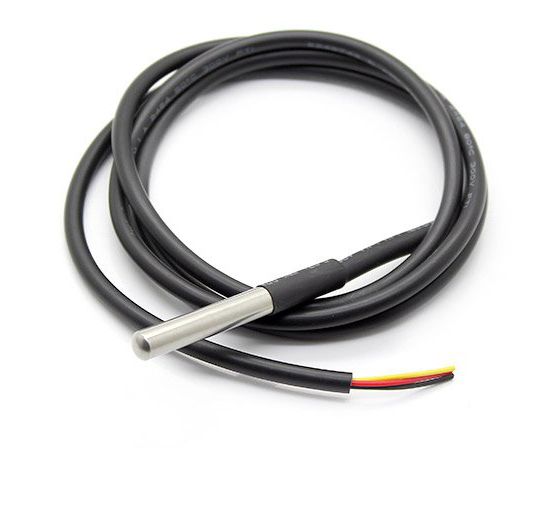
\includegraphics[scale=0.35]{hardware/ds18b20.jpg}
                    \caption{Sensor sumergible de temperatura - DS18B20}
                    \label{SensorTemp}
                \end{figure}
                
            \paragraph{Sensor de pH de líquidos:}Sensor electroquímico de pH\footnote{ Medida de acidez o alcalinidad de una disolución}, compuesto por un electrodo sumergible y una placa electrónica denominada sonda de pH (pH probe), los cuales transducen la actividad química del ion de hidrógeno en una señal eléctrica. (Figuras \ref{BoardPh} y \ref{phElectrode})
                
                \par Se procedió a adquirir un sensor con precio acorde al presupuesto de los alumnos. Se describen a continuación las características del modelo elegido:
                
                \begin{itemize}
                    \item Modelo: phMeter
                    \item Voltaje de funcionamiento : 5V
                    \item Comunicación: Analógica, cuenta con 6 pines. Conector tipo BNC
                    \item Precisión: ± 0.1pH, tomando valores de 0-14 pH
                    \item Temperatura de trabajo: 0 - 60ºC
                    \item Tiempo de Respuesta: 1 minuto
                \end{itemize}
                
                \begin{minipage}{0.95\textwidth}
                    \begin{center}
                    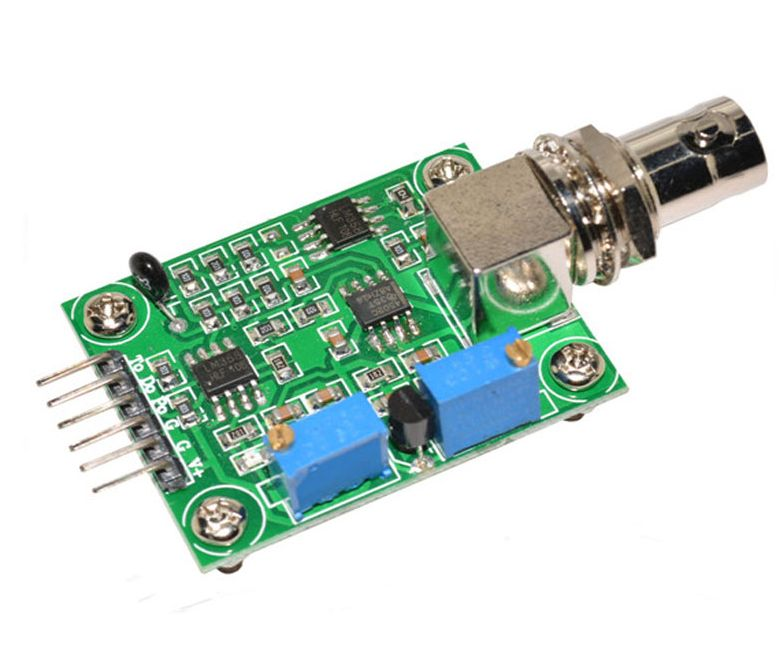
\includegraphics[scale=0.25]{hardware/phmoduloplaca.jpg}
                    \captionof{figure}{Placa sonda de pH}
                    \label{BoardPh}
                    \end{center}
                \end{minipage}
                
                \begin{minipage}{0.95\textwidth}
                    \begin{center}
                    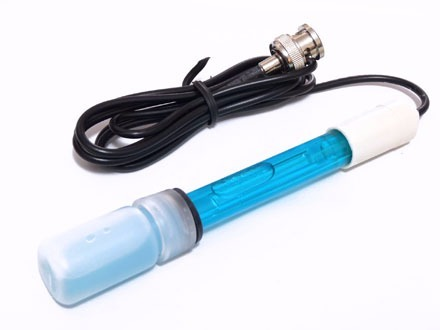
\includegraphics[scale=0.35]{hardware/electrododepH.jpg}
                    \captionof{figure}{Electrodo de pH}
                    \label{phElectrode}
                    \end{center}
                \end{minipage}
                
            \paragraph{Sensor de temperatura y humedad ambiental:}Sensor digital que permite realizar mediciones ambientales de temperatura y humedad relativa. Dados los condicionamientos antes planteados, el funcionamiento digital y las buenas prestaciones, se eligió el modelo de bajo costo DHT11 (Figura \ref{SensorDHT11}), sus características son descritas a continuación:
                \begin{itemize}
                    \item Modelo: DHT11
                    \item Fabricante: Adafruit
                    \item Voltaje de funcionamiento: 3V - 5V DC
                    \item Comunicación: Digital. Posee cuatro pines: VDD, Data, Idle, GND.
                    \item Rango de medición de temperatura: 0 a 50 °C
                    \item Precisión de medición de temperatura: ±2.0 °C
                    \item Resolución Temperatura: 0.1°C
                    \item Rango de medición de humedad: 20\% a 90\% RH
                    \item Precisión de medición de humedad: 4\% RH
                    \item Resolución Humedad: 1\% RH
                    \item Tiempo de sensado: 2 seg
                \end{itemize}
                
                \begin{figure} [h]
                    \centering
                    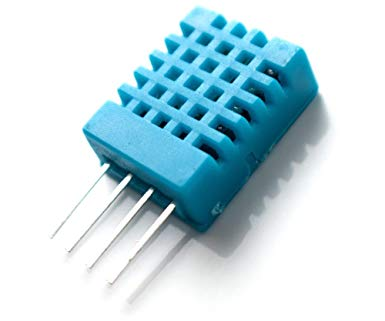
\includegraphics[scale=0.35]{hardware/dht11_.jpg}
                    \caption{Sensor de temperatura y humedad ambiente DHT11}
                    \label{SensorDHT11}
                \end{figure}

        
\section{Diseño}
    \par En las siguientes secciones se analiza y define la estrategia utilizada para abordar el desarrollo de este componente.
    
    \subsection{Lista de elementos}
        \begin{itemize}
            \item 6 sensores digitales de temperatura sumergibles DS18B20 con 2 metros de extensión por cable
            \item 1 sensor digital de temperatura y humedad ambiente Adafruit DHT11
            \item 1 sensor de pH analógico ( Electrodo y Plaqueta controladora)
            \item 1 Conversor Analógico / Digital (Arduino\textsuperscript{\textregistered} Uno)
            \item 1 Raspberry\textsuperscript{\textregistered} Pi 3 B+
            \item Resistencias electrónicas (4.7 k$\Omega$, 10 k$\Omega$)
            \item Protoboard con cables
            \item Fuente de alimentación microUSB 5v 2.1A
            \item Memoria Micro SD Clase 10 16GB
        \end{itemize}
        
    \subsection{Consideraciones previas}
        \par En este apartado se describen restricciones inherentes al funcionamiento del sistema que debieron ser consideradas para el diseño del mismo. Cada una, se detalla, justificando la decisión de diseño que se optó.
        
        \paragraph{Medición de pH:} 
            La obtención de este valor se realiza mediante el sensor electroquímico antes mencionado. Este requiere de al menos 2 minutos para estabilizar el resultado (medición) obtenido debido a cuestiones inherentes al funcionamiento del mismo. Por lo cual, el intervalo de medición no podrá ser inferior a este lapso mínimo.
            
            \par Respecto de la variación de las mediciones de pH con la temperatura, (M. E. Mohammd Ali y O. A. Razag Sharif, 2015) expresa que la medición es afectada de dos maneras. Por un lado, al valor de pH de la solución, cuya corrección directa no puede ser realizada, dado que cada muestra de pH tiene una relación\footnote{Coeficiente de temperatura de la solución  $ = \Delta pH/ ^{\circ}C $} entre pH y temperatura única. Sin embargo, una compensación de pH debe ser realizada a través de una calibración utilizando soluciones \textit{buffers} de pH estándares. Por otro lado, al efecto de la temperatura sobre la sensibilidad del electrodo de pH, el cual puede ser corregido y cuya desviación depende de cada electrodo. El fabricante del electrodo utilizado en este desarrollo provee la Tabla \ref{tablePhvsTemp} de desvíos. 
            
            \begin{figure}[h] 
                \centering
                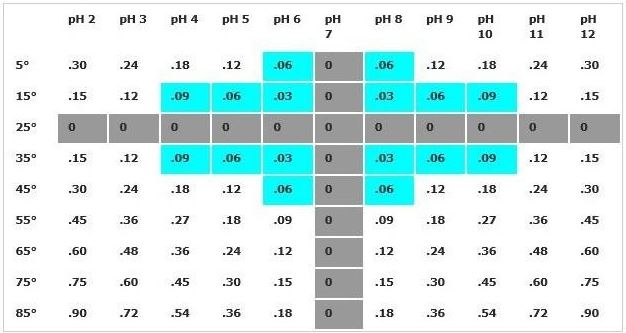
\includegraphics[scale=0.9]{errorMedicionPh.jpg}
                \caption{Error de medición de pH respecto a la temperatura de la solución}
                \label{tablePhvsTemp}
            \end{figure}
            
            \par Para este proyecto, el intervalo de mediciones de pH será de 2 minutos o superior (siendo el usuario quien define esto según el método de enfriamiento de muestras que utilice) asumiendo así el correspondiente error. En forma adicional, el error debido al desvío por la temperatura durante la medición de pH es ajustado utilizando un sensor sumergible de temperatura destinado a este propósito, junto a la Tabla \ref{tablePhvsTemp}.
        
        \paragraph{Medición de temperatura:} 
            Debido a que el objeto involucrado en la medición es un líquido, se opta por un sensor de temperatura sumergible.
        
            
        
        \paragraph{Almacenamiento:} 
             Son requeridos aproximadamente 5 gigabytes de espacio de almacenamiento en memoria SD para la instalación del sistema operativo y las herramientas necesarias para el funcionamiento del componente.
            
            \par La mínima capacidad suficiente para satisfacer el requerimiento de almacenamiento antes descrito es de 8 gigabytes. Siendo considerado el espacio libre en esta  capacidad, podrán ser almacenadas numerosas experiencias debido a que no es utilizado más de un megabyte para cada una.
            
            \par En conclusión, una limitante de almacenamiento no será objeto de análisis para el desarrollo del prototipo.
            
        \paragraph{Desconexión de sensores:} 
             Ante la posible desconexión de algún o algunos sensores, el sistema debe ser capaz de identificarlo/s. Luego, reportar el error para considerar el desperfecto para próximos experimentos y evitar incorporar el valor medido por dicho/s sensor/es a las estadísticas de funcionamiento. Dado que se plantea al sistema como una herramienta de asistencia al productor, se opta por no cancelar el experimento bajo esta situación debido a los costos de la materia prima involucrada.
            
            
    \subsection{Diseño del componente}
            \par En cuanto al diseño de esta estación de recolección de datos, fueron identificadas las siguientes subcapas: Subcapa de Software y Subcapa de Hardware.
            
            \subsubsection{Subcapa de Software}
                \par El sistema operativo a ser utilizado para el Raspberry\textsuperscript{\textregistered} será Raspbian, una distribución basada en Debian Linux provista por el fabricante de la placa.
                
               \par El desarrollo de las funcionalidades de software se implementarán bajo el lenguaje Python, elegido como primer alternativa. El mismo cuenta con una numerosa comunidad de desarrolladores, librerías y es recomendado por el sitio oficial de Raspberry\textsuperscript{\textregistered} (Raspberry\textsuperscript{\textregistered} Official Page, 2018) para la programación con GPIO.
                
                \par Para la gestión de los datos, será empleado el motor de base de datos MySQL. Se justifica esta elección por su simpleza de uso, mínimos requerimientos para un correcto funcionamiento y la existencia de herramientas de interacción con scripts en lenguaje Python.
                
                \par Respecto del funcionamiento del componente, un batch se ejecuta mediante comandos bash del sistema al que se le proveerán los parámetros necesarios para el proceso de obtención de datos. Se repetirán ciclos de muestreo, ejecutando en cada iteración las funciones necesarias para los fines requeridos:
                    
                    \begin{itemize}
                        \item Obtención de datos de sensores: Desarrollo de una función específica para cada sensor. De esta manera, se abordan de manera precisa y eficaz los posibles inconvenientes (bugs) que puedan ser identificados.
                        
                        \item Inserción de datos en la Base de Datos: Los datos obtenidos en cada secuencia de medición se insertan en la base de datos a partir de un identificador (Id) proporcionado como parámetro de la función.
                    \end{itemize}
                
                \paragraph{Diagrama de Base de Datos:} La Figura \ref{fig:DiagramaBdRasp} ubicada en el Anexo, presenta el diagrama de base de datos utilizado. El mismo, consiste de tres tablas relacionadas mediante claves foráneas (foreign keys): \textit{Maceración}, \textit{Experimento} y \textit{SensedValues}. 
                
                
            \subsubsection{Subcapa de Hardware} 
                \par En la Figura \ref{fig:EsquemaHardware} del Anexo, se presenta un esquema simplificado de conexiones en esta subcapa. En el mismo se encuentran identificadas las entradas (sensores y conversor) y la salida (API REST) del Raspberry\textsuperscript{\textregistered} Pi.
                
                
                
                \par Para la conversión analógico digital, requerida para la señal del sensor de pH, se utiliza un Arduino\textsuperscript{\textregistered} Uno en modo esclavo para utilizar su DAC interno de 10 bits.
        
    
\section{Implementación del diseño}

    \subsection{Subcapa de software}
        \par El siguiente diagrama de flujo (Figura \ref{FlujoPython}), muestra el funcionamiento del código desarrollado utilizando lenguaje Python cumpliendo las funcionalidades mencionadas en el apartado de diseño.

        \begin{figure}[H]
            \centering
            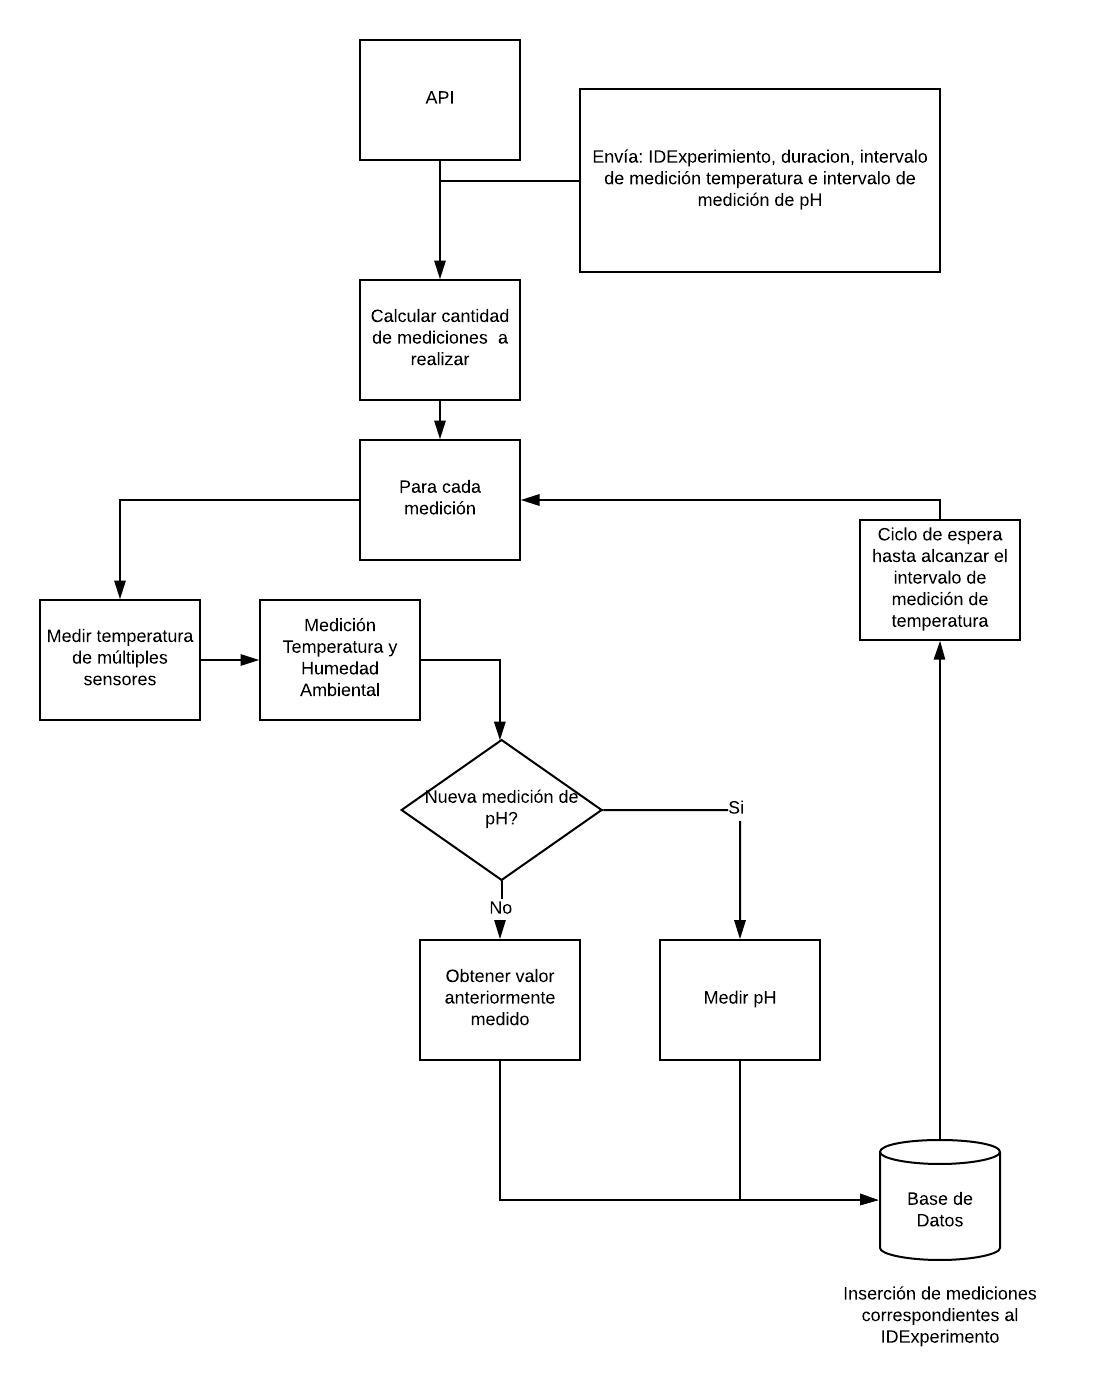
\includegraphics[scale=0.8]{hardware/DiagramadeFlujoPython.jpeg}
            \caption{Diagrama de flujo del funcionamiento del software }
            \label{FlujoPython}
        \end{figure}

\section{Subcapa de hardware}
    \par En las siguientes subsecciones se muestran los diagramas de conexión de cada sensor con la placa Raspberry, siguiendo el diseño general de la la Figura \ref{fig:EsquemaHardware} del Anexo.

    \subsection{Conexión sensor de pH}
        \par A continuación, se muestra el diagrama de conexión del sensor de pH (Figura \ref{fig:ConexionSensorpH}), conformado por el sensor electroquímico, electrodo y "sonda de pH", antes mencionado. Este último, se encuentra conectado a una placa Arduino\textsuperscript{\textregistered} UNO que realiza la función de conversor Analógico-Digital enviando los datos analógicos obtenidos por el sensor como una señal digital al Raspberry\textsuperscript{\textregistered} mediante conexión Serial USB.
        
        \begin{figure}[h]
            \centering
            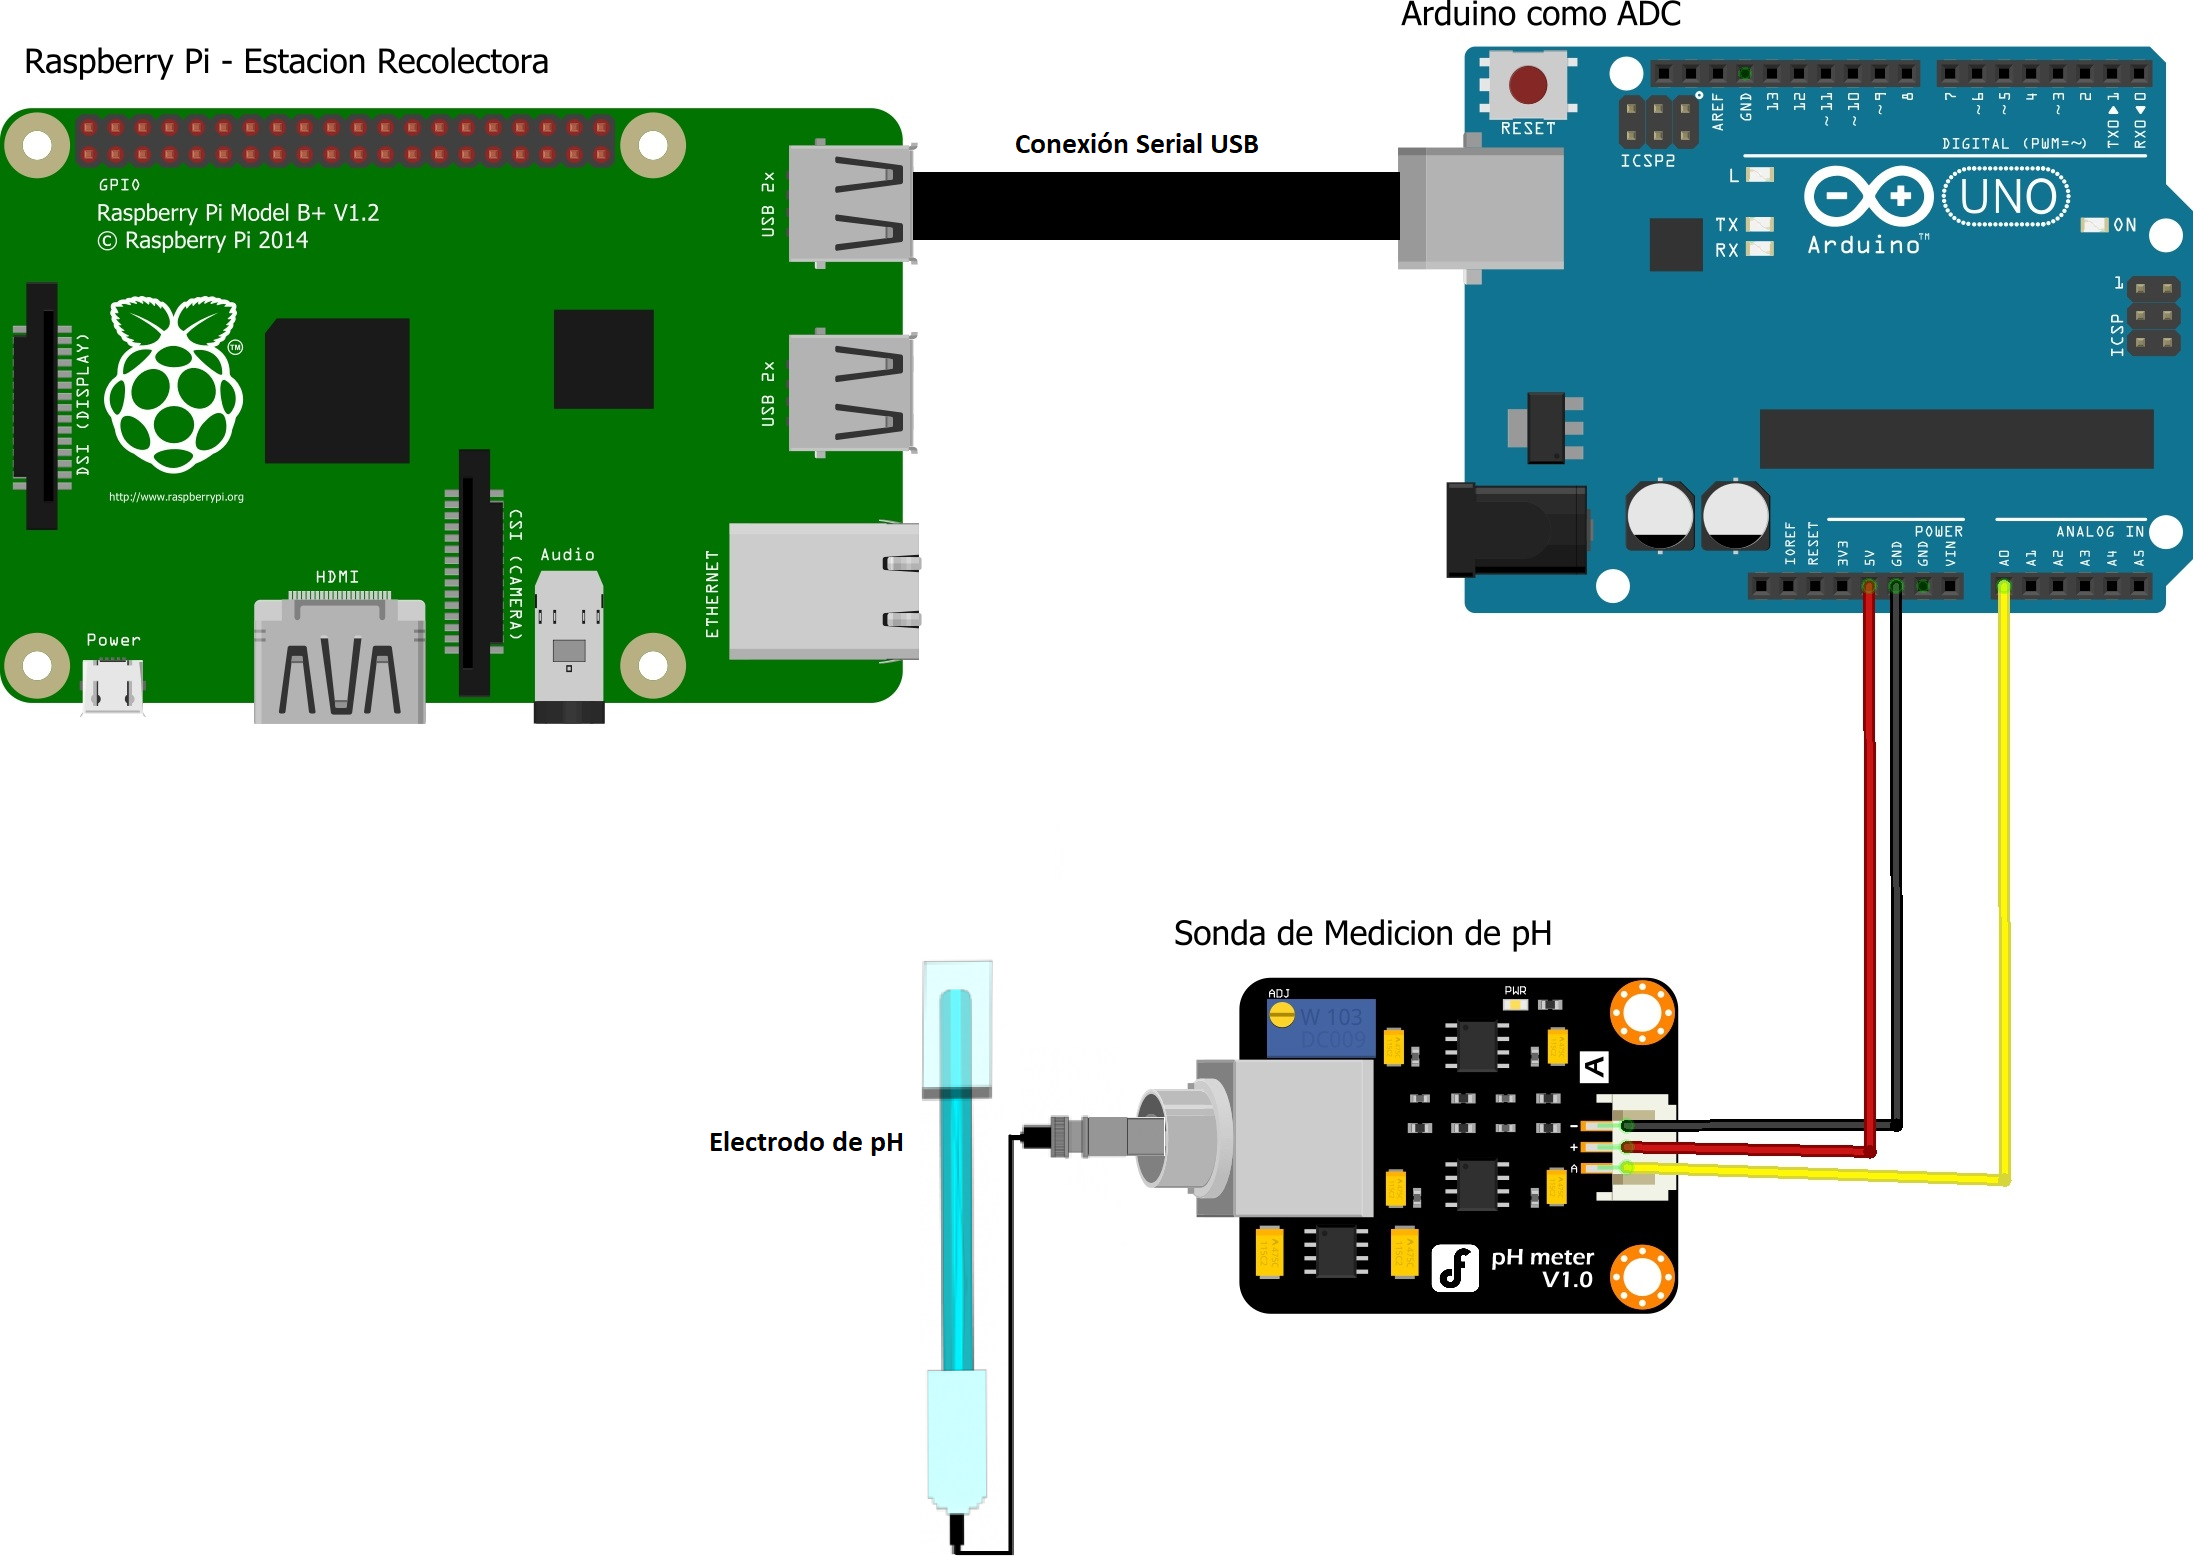
\includegraphics[scale=0.25]{hardware/DiagramaSensordepH_bb2.jpg}
            \caption{Diagrama de conexión del sensor de pH}
            \label{fig:ConexionSensorpH}
        \end{figure}

    \subsection{Conexión sensor de temperatura sumergible}

        \par Este sensor requiere la conexión de un resistencia de $4.7k\Omega$ entre el pin de datos (Data) y el de corriente continua (VDD). En forma adicional, este sensor incorpora la posibilidad de conexión de múltiples sensores en serie mediante el bus I2C\footnote{Bus desarrollado por Philips\textsuperscript{\textregistered} para envío de datos en serie entre un circuito maestro y uno o varios esclavos}. Bajo esta dinámica, cada uno dispone de un código de identificación único permitiendo de esta manera ser identificado de forma univoca. En la figura \ref{fig:ConexionTemperatura} se presenta el diagrama de conexión de estos sensores.
        
        \begin{figure}[h]
            \centering
            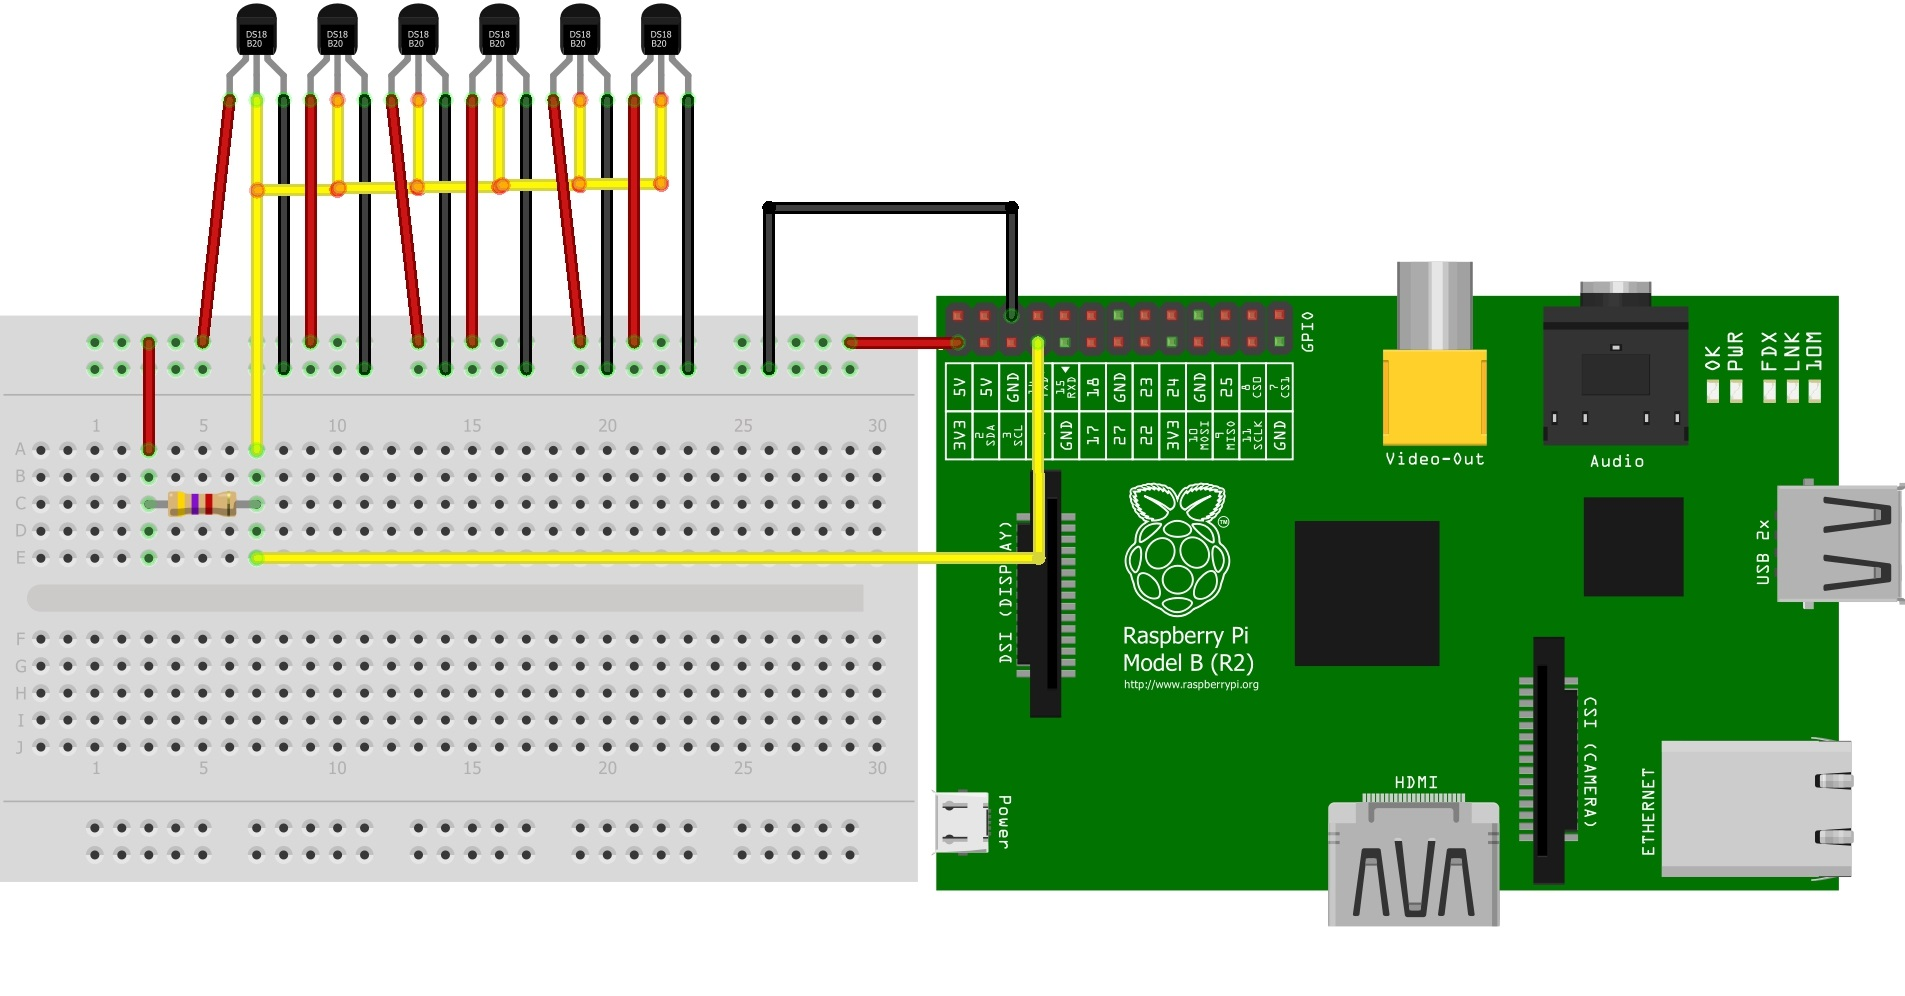
\includegraphics[scale = 0.8]{DiagramaSensordeTemp_bb.jpg}
            \caption{Diagrama de conexión de los sensores de temperatura}
            \label{fig:ConexionTemperatura}
        \end{figure}
        
    \subsection{Conexión sensor temperatura y humedad ambiental}
        \par Este sensor, al igual que el anterior, requiere la conexión de los pines de corriente continua (VDD) y el de datos (Data) mediante una resistencia de $4.7k\Omega$. A continuación se muestra la figura \ref{fig:EsquemaDHT11} con el esquema de conexión.
        
        \begin{figure}[h]
            \centering
            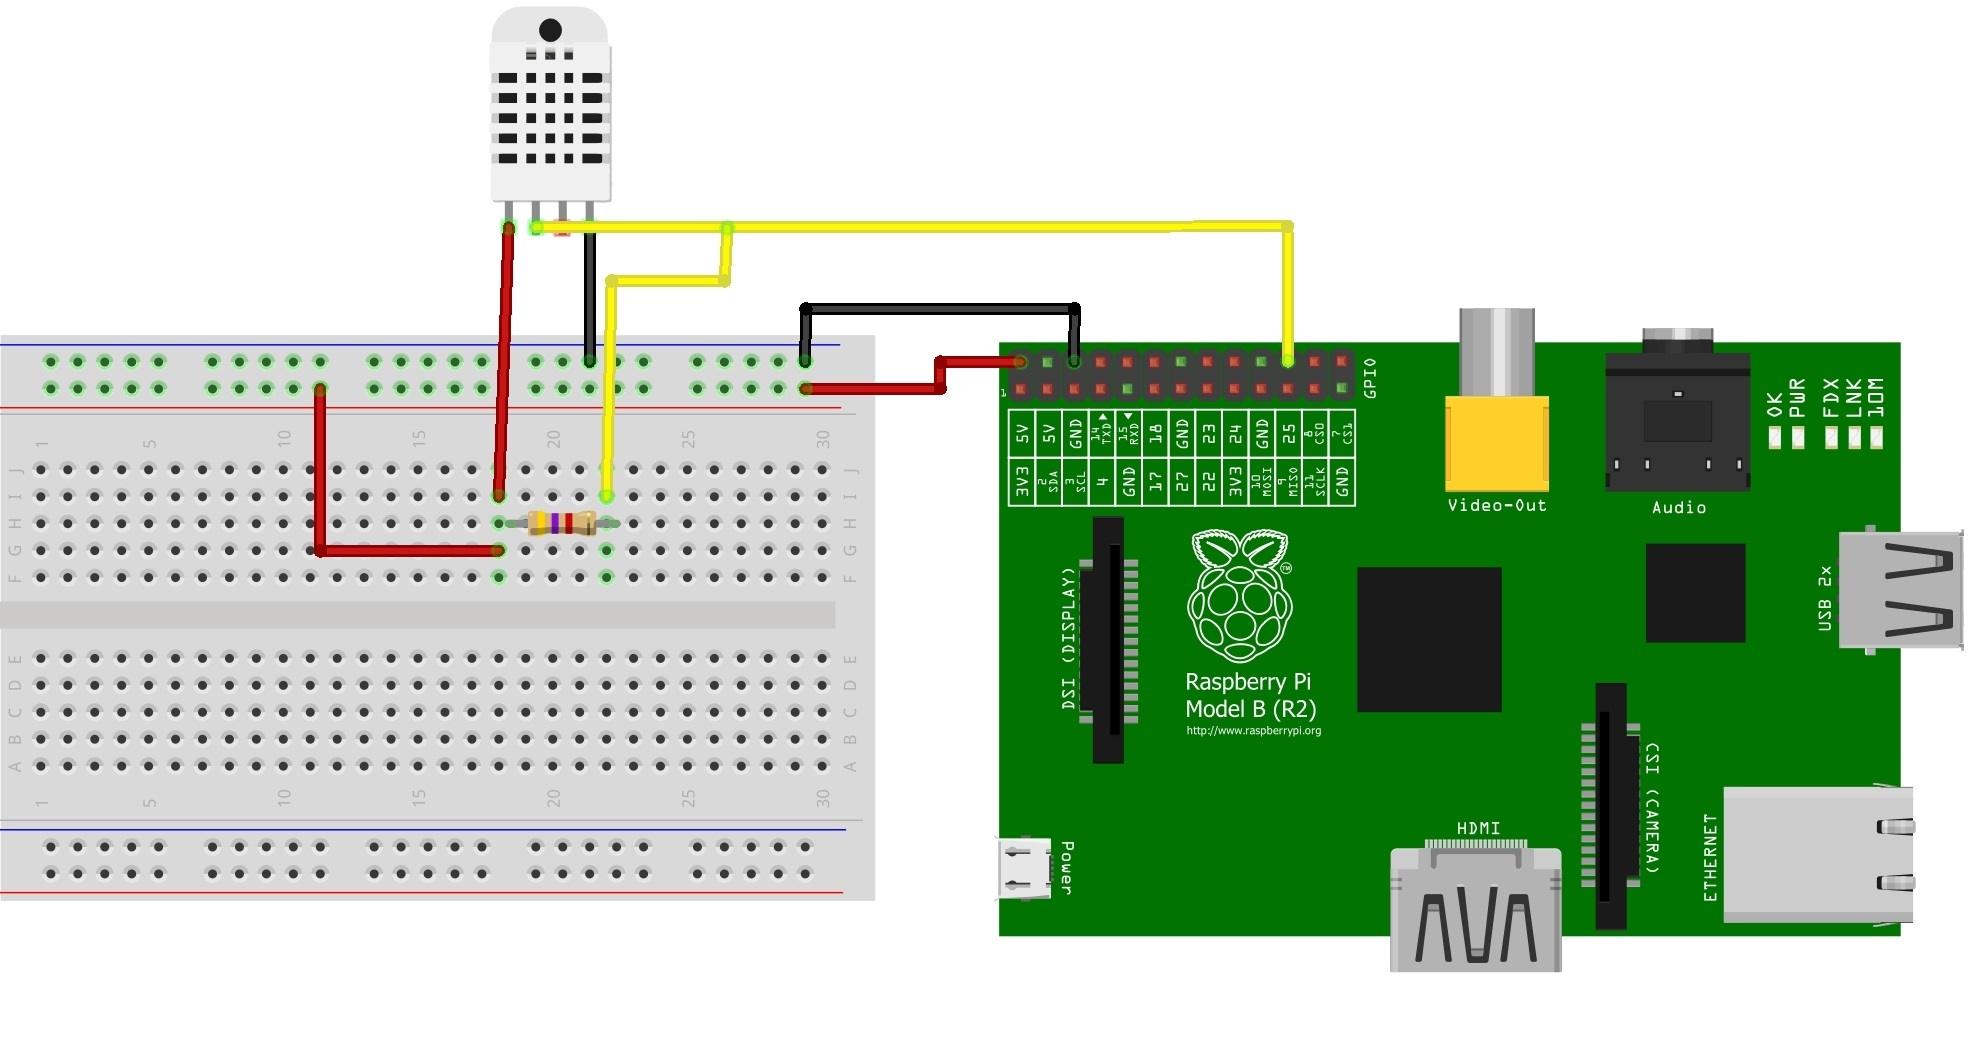
\includegraphics[scale = 0.8]{DiagramaSensorDHT11_bb.jpg}
            \caption{Diagrama de conexión del sensor DHT11}
            \label{fig:EsquemaDHT11}
        \end{figure}

\section{Ensamble completo}
\begin{minipage}{0.95 \textwidth}
    \par Finalmente, se exhibe una imagen fotográfica de la estación de recolección de datos conectada e integrada con todos sus sensores (Figura \ref{fig:EsquemaCompletoHardware}).\\
\end{minipage}
\begin{minipage}{0.95 \textwidth}
    
        \centering
        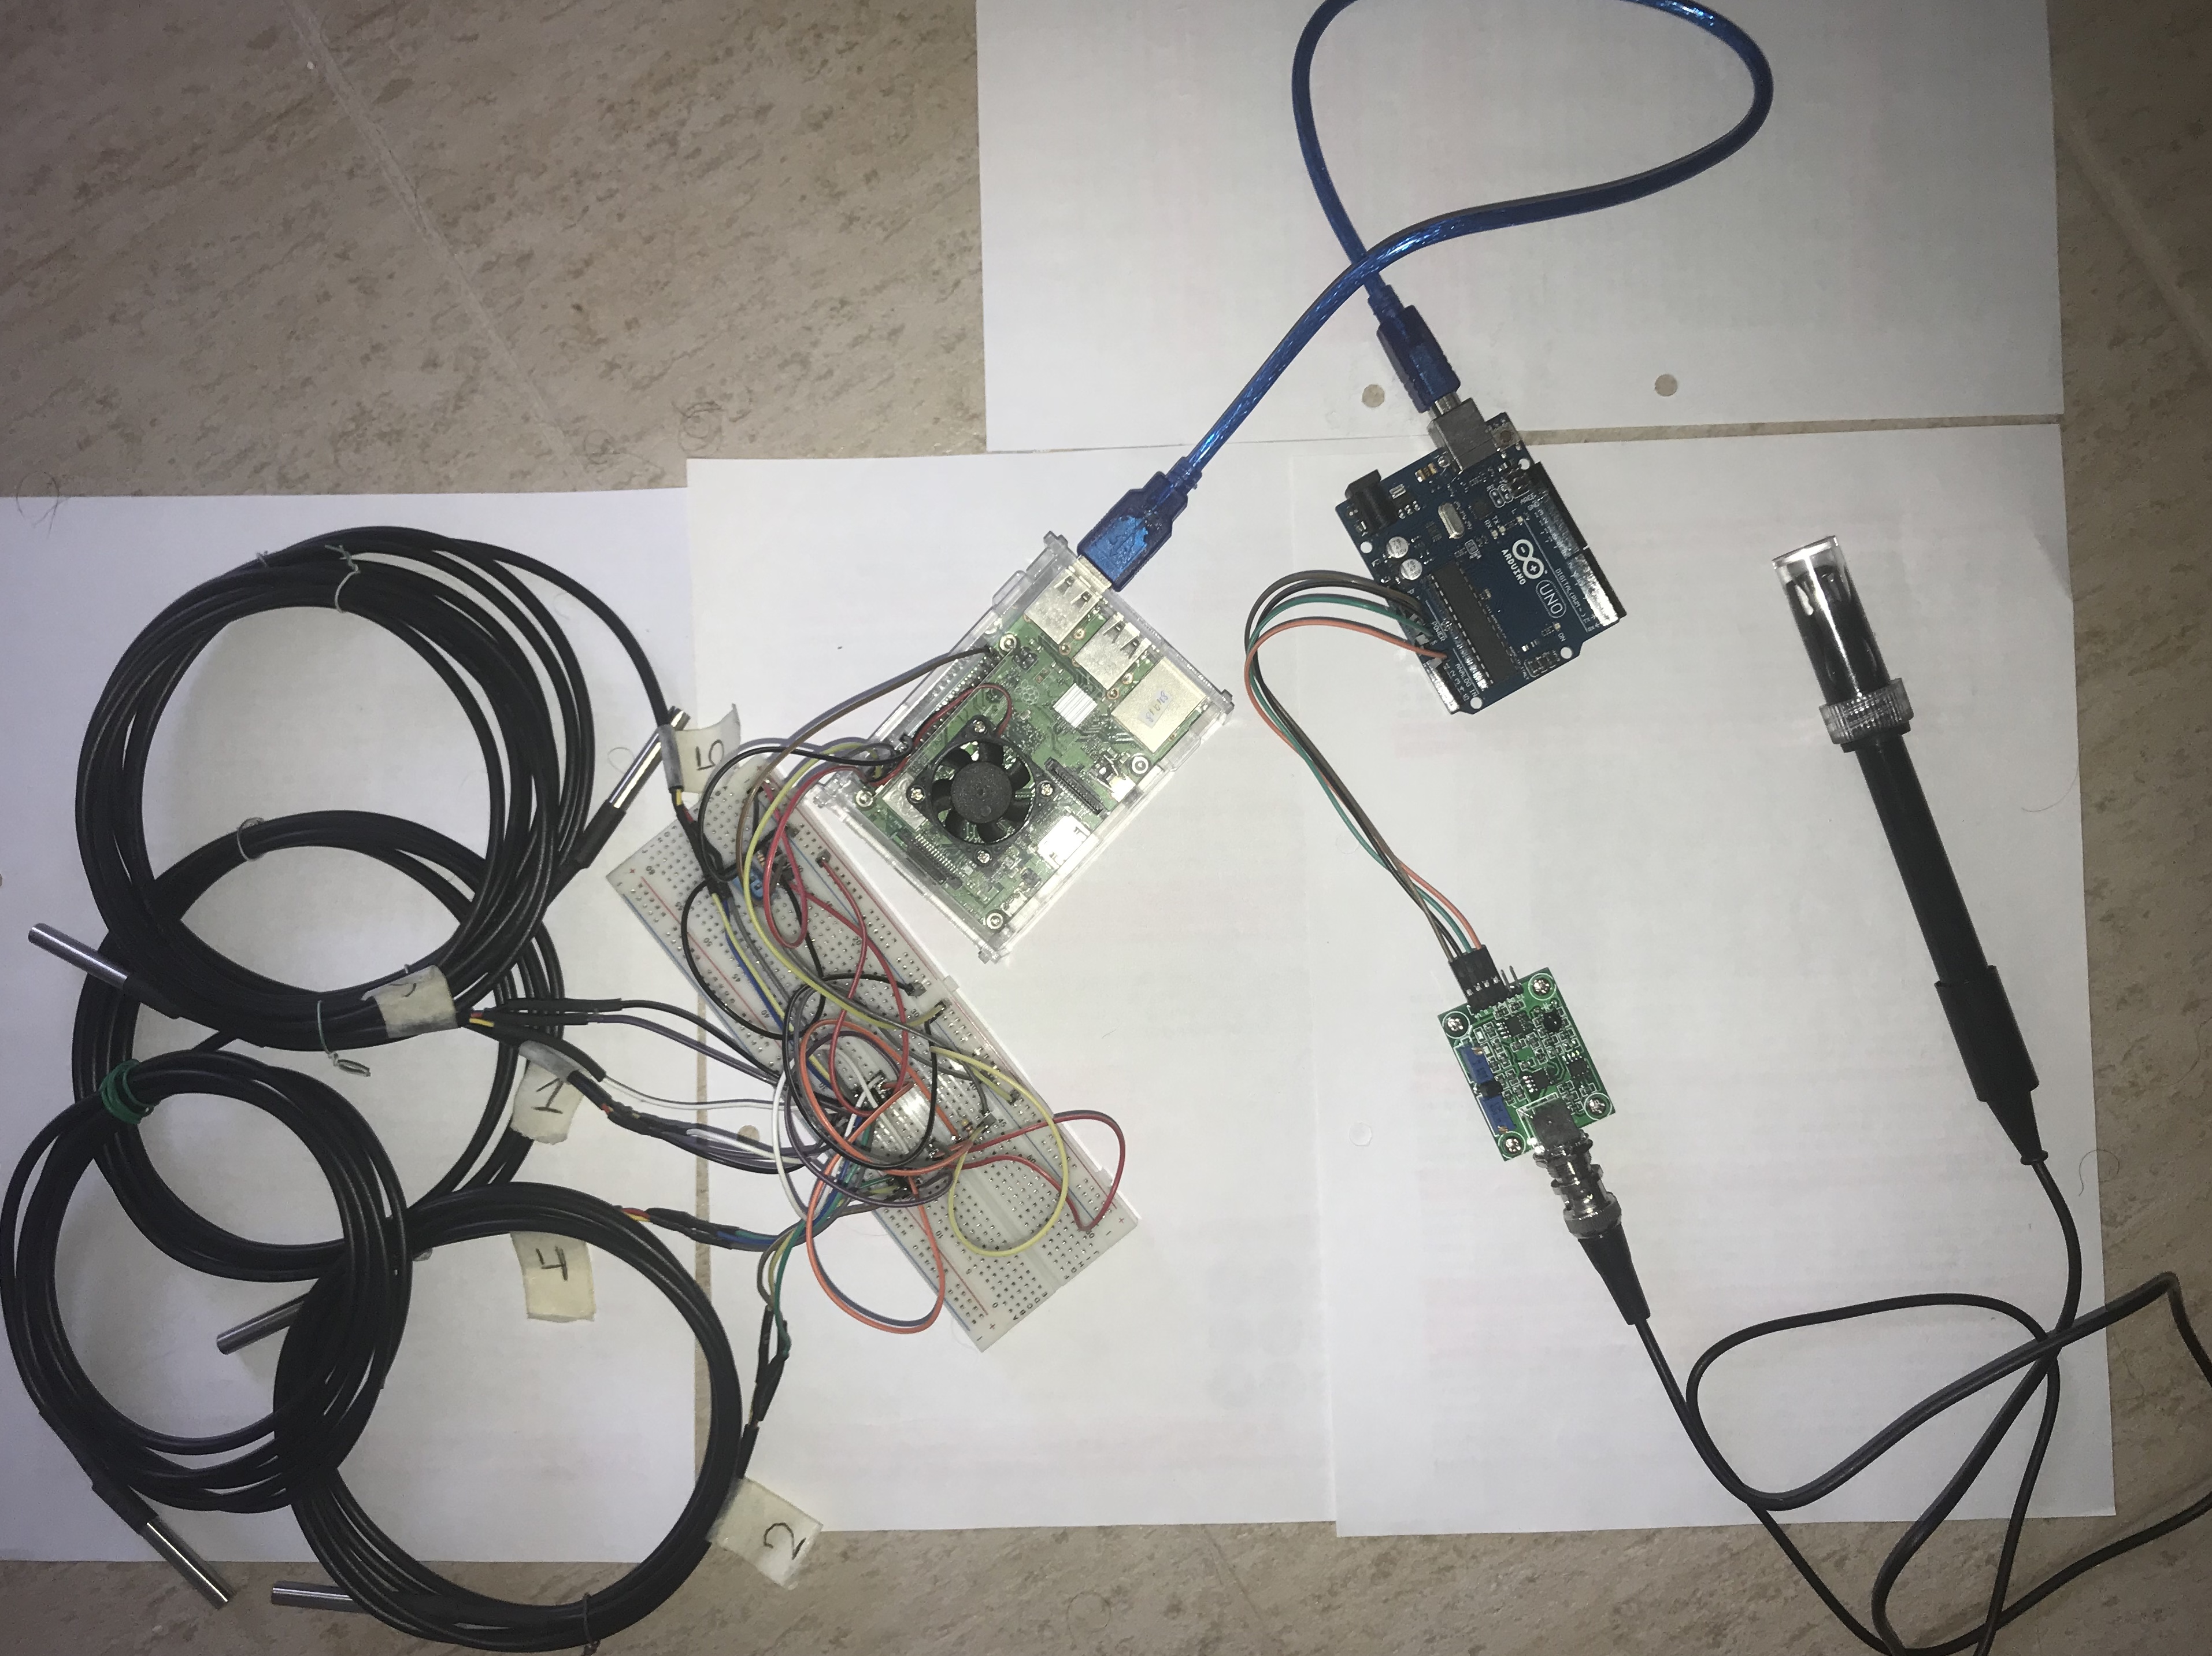
\includegraphics[scale=0.1]{hardware/SistemaEnsamblado.jpeg}
        \captionof{figure}{Fotografía de la estación de recolección de datos}
        \label{fig:EsquemaCompletoHardware}
    
\end{minipage}